\chapter{Theory}
In this section, the theoretical modelling of the bicycle and the data driven Min-Max MPC is discussed.

Since the objective of this research is to simply balance the bicycle, a simple kinetic model is sufficient for this purpose. We use to models and compare between them in terms of control and balance.
The difference between both models is considering the fork angle.

\section{Bicycle Model}
	To model the bicycle, we 
	
	
	
	
	Bicycles:
	
	Models \cite{astrom}
	%\math
	
	* Consider with fork angle
	
	* Write equation and code
	\\
	
	\textbf{Simple Second-Order Models}:
	
	\begin{itemize}	
		\item Fork Angle:\\
		$\varphi_f = \varphi - \delta \cos \lambda$\\
		$\varphi_f =  \delta \sin \lambda$\\		
		$F_f = \frac{amV^2}{b^2} \delta_f = \frac{amV^2 \sin \lambda}{b^2} \delta.$\\
		$T - \left(F_f + N_f(\varphi_f)\right)c \sin \lambda = 0.$\\
		
		$T - \frac{acmg \sin \lambda}{b} \varphi - \frac{acm \sin \lambda}{b^2} \left(V^2 \sin \lambda - bg \cos \lambda\right) \delta = 0$
		\\
		$V_{sa} = \sqrt{bg \cot \lambda}$
		\\
		$\delta = k_1(V)T - k_2(V)\varphi,$
		\\
		$k_1(V) = \frac{b^2}{\left(V^2 \sin \lambda - bg \cos \lambda\right) mac \sin \lambda},$
		\\
		$k_2(V) = \frac{bg}{V^2 \sin \lambda - bg \cos \lambda}.$
		\\
		Turn into codes later
		\item Self-Stabilization
		\item Manual Control
		\item Gyroscopic Effects
		\item Rear-Wheel Steering\\
		Later
		\item Effects of Rider Lean: Irrelevant
	\end{itemize}
	
	\textbf{Linear and Non-Linear Fourth order Models}
	
	
	
	
	\textbf{Morlock's 2.40 equation:}
	
	State-space representation:
	
	\begin{equation}
		\ddot{\varphi} - \frac{g}{h} \varphi = \frac{av \sin \lambda}{hl} \dot{\delta} + \frac{\left(v^2 h - ar_\tau g\right) \sin \lambda}{h^2 l} \delta.
	\end{equation}
	
	
	\[
	\begin{bmatrix} 
		\dot{\phi} \\ 
		\ddot{\phi} \\ 
		\dot{\delta} 
	\end{bmatrix} 
	=
	\begin{bmatrix} 
		0 & 1 & 0 \\ 
		\frac{g}{h} & 0 & \frac{\left(v^2 h - ar_\tau g\right) \sin \lambda}{h^2 l} \\ 
		0 & 0 & 0 
	\end{bmatrix} 
	\begin{bmatrix} 
		\phi \\ 
		\dot{\phi} \\ 
		\delta 
	\end{bmatrix}
	+
	\begin{bmatrix} 
		0 \\ 
		\frac{av \sin \lambda}{hl} \\ 
		1 
	\end{bmatrix} 
	\dot{\delta}.
	\]
	
	
	Generate data using LQR feedback control:
	
	Using Bryson's rule to set Q and R:
	
	\begin{equation}
		Q = \begin{bmatrix}
			1 & 0 & 0 \\
			0 & 1 & 0 \\
			0 & 0 & 1 
		\end{bmatrix}, 
		R = \begin{bmatrix}
			1
		\end{bmatrix}	
	\end{equation}



\section{Data-Driven Min-Max MPC}
To formulate our problem, we represent the system using \[x_{t+1} = A_s x_t + B_s u_t + \omega_t,\] where 

	\begin{figure}
		\centering
		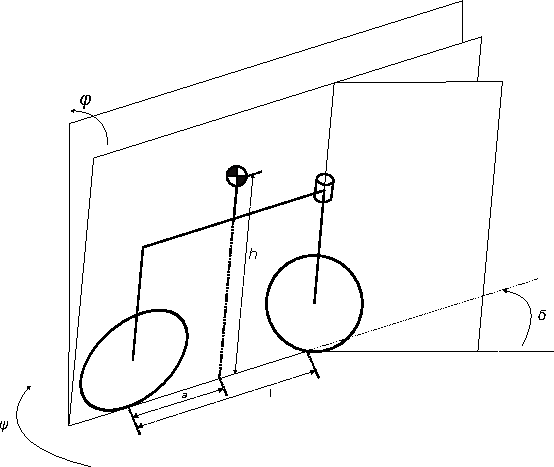
\includegraphics[width=0.7\linewidth]{figures/minibike/model.pdf}
		\caption{A Kinetic no-fork model of the bicycle}
		\label{fig:model}
	\end{figure}